\documentclass{article}
\usepackage[utf8]{inputenc}
\usepackage{pdflscape}
\usepackage{graphicx}
\usepackage{hyperref}
\usepackage{longtable}
\usepackage{array}

\title{PLD Agile: Agile Development Report}
\author{
    Mark Beckmann, Back-End Developer \& Product Owner \\
    Evann Guillot, Back-End Developer \\
    Noham Martin, Back-End Developer \\
    Tim Morel, Front-End Developer \\
    Marie Roulier, Full-Stack Developer \& Scrum Master \\
    Hugo Warin, Full-Stack Developer \\
    Zyad Haddad, Front-End Developer
}
\date{Group: H4132 \\ Department: Computer Science \\ University: INSA Lyon}

\begin{document}

\maketitle

\begin{figure}[ht]
\centering

\includegraphics[width=0.5\textwidth]{uni_logo.jpg}
\caption{University Logo}
\end{figure}

\newpage
\tableofcontents
\newpage

\section{Introduction}
This report documents the Agile development process of the PLD Agile project. The project's goal is to develop an application for optimizing delivery tours in urban settings using bicycles. Embracing Agile and SCRUM methodologies, the focus is on iterative development, robust team collaboration, and high adaptability.

\section{First Iteration Report}

\subsection{Use Case Diagram}
\begin{figure}[ht]
\centering
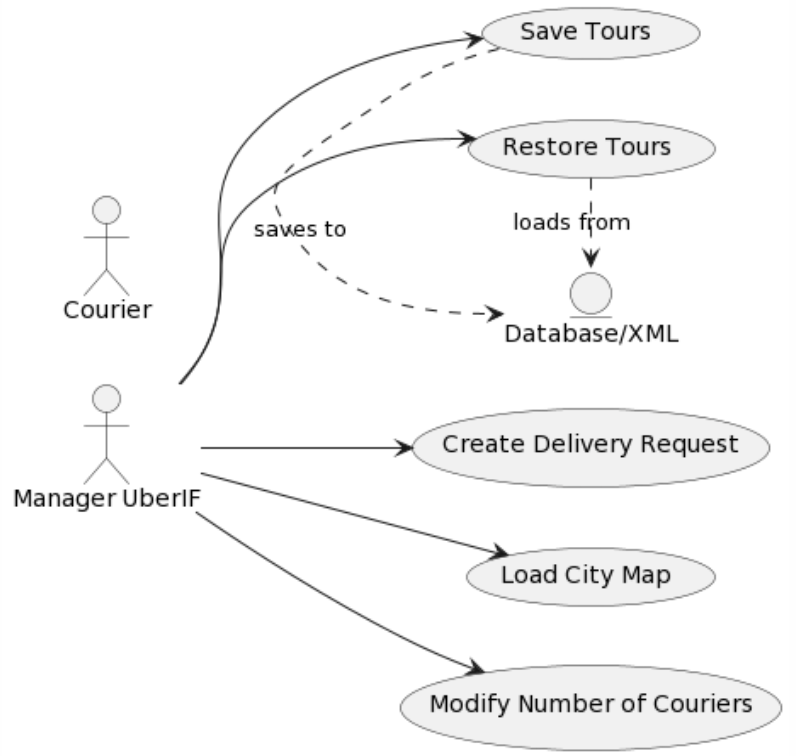
\includegraphics[width=0.8\textwidth]{useCase.png}
\caption{Use Case Diagram}
\end{figure}
By Manager UberIF, we mean the user that get incoming delivery requests, calculates routes from the warehouse and that manages the couriers.

\subsection{Main Success Scenario Description}
\begin{longtable}{|m{5cm}|m{10cm}|}
\hline
USE CASE & Main Success Scenario \\
\hline
Create Delivery Request & 
1. Manager logs into the system
2. Manager selects the option to create a new delivery request
3. System displays the form to enter necessary details (courier, time window, destination address)
4. Manager fills in the form and submits it
5. System checks and validates data
6. System creates the delivery request
7. System initiates the process of finding an available courier and computing the best tour 
8. System displays the map with the best tour for delivery \\
\hline
Load City Map & 1. Manager logs into the system 2. Manager selects the option to load the city map 3. System gets all the necessary information from an XML file 4. System confirms successful loading of the map \\
\hline
Modify Number of Couriers & 1. Manager logs into the system 2. Manager clicks on “+” or “-” to modify the number of available couriers 3. System adjusts the number of couriers \\
\hline
Save Tours & 1. Manager logs into the system 2. Manager clicks on saving the tours running at the moment 3. System saves tours details to an XML file 4. System acknowledges successful saving of the tour  \\
\hline
Restore Tours & 1. Manager logs into the system 2. Manager clicks on restoring the tours 3. Manager chooses the tours they want to restore 4. System retrieves and displays the selected tour details  \\
\hline
\end{longtable}

\subsection{Description of All Use Cases}
\begin{longtable}{|m{5cm}|m{10cm}|}
\hline
USE CASE & DESCRIPTION \\
\hline
Create Delivery Request & Allows the manager to create a new request and input details of the delivery. The manager has to select a courier, a 1-hour time window, and the destination intersection. This will enable the computing of the best tour by the computer. Then, the departure and arrival times, as well as the tour, are displayed. For now, to create a delivery request the Manager UberIF has to click on the intersections to add them to a tour. The form will be implemented in the next iteration. To be further improved.  \\
\hline
Load City Map & Display the map of the chosen city on the screen. The map is responsive, as the entire application. Has been implemented.     |
| Modify Number of Couriers | Modify the number of active couriers in the system. Has been implemented.  \\
\hline
Modify Number of Couriers & Modify the number of active couriers in the system. Has been implemented.  \\
\hline
Save Tours & Store in a file all the tours done in the city, as well as the departure and arrival time, corresponding courier, and the destination address. Analyzed, not implemented yet. \\
\hline
Restore Tours & Retrieve and load from file old tours and corresponding information, departure and arrival time as well as destination address, and display them. Analyzed but not implemented yet. \\
\hline
\end{longtable}

\subsection{Class and Package Diagrams}
The aim of this diagram is to explain how we want to build our software to answer the client needs. It is important to note that this diagram constantly evolves and therefore only should be used to understand the general idea of how our software is structured. It is not the actual nor final version and doe not exactly explain all classes and packages.
\\
This diagram is organized into several packages, which group related classes and interfaces that interact with each other to perform various functions within the application.

\subsubsection{Description and Explanation of the Diagram:}
\begin{itemize}
    \item \textbf{Models Package:} Contains the core data structures and logic.
    \begin{itemize}
        \item \textbf{Delivery:} Represents a delivery request, including location, time window, and assigned courier.
        \item \textbf{CityMap:} Holds the graph data structure of the city, with intersections and road segments.
        \item \textbf{Courier:} Stores information about each courier, including their current tour.
        \item \textbf{Tour:} Manages the sequence of deliveries and the computation of the optimal route.
    \end{itemize}
    \item \textbf{Views Package:} Deals with the user interface and presentation logic.
    \begin{itemize}
        \item \textbf{Window:} The main window of the application.
        \item \textbf{GraphicalView:} Responsible for rendering the map and tours visually.
        \item \textbf{MouseListener, KeyboardListener, ButtonListener:} Handle user inputs.
    \end{itemize}
    \item \textbf{Controllers Package:} Manages the application flow and responds to user actions.
    \begin{itemize}
        \item \textbf{Controller:} The main controller that orchestrates the application's behavior.
        \item \textbf{ListOfCommands:} Maintains a list of commands for undo/redo functionality.
        \item \textbf{Command:} An abstraction for actions that can be performed, such as adding or removing a delivery.
    \end{itemize}
    \item \textbf{XMLMapParser:} A utility class for parsing the city map from an XML file.
\end{itemize}

\textbf{Architecture and Design Patterns:}
\begin{itemize}
    \item The architecture follows the \textbf{Model-View-Controller (MVC)} pattern, separating concerns and allowing for modular development and testing.
    \item \textbf{Observer pattern} is used within the Models package, allowing views to react to changes in the model.
    \item The \textbf{Command pattern} is implemented in the Controllers package, encapsulating actions as objects, enabling sophisticated control structures such as undo/redo.
    \item \textbf{State pattern} seems to be used for managing different states of the application, such as initial, address, and delete states.
\end{itemize}

\begin{landscape}
\begin{figure}[]
\centering
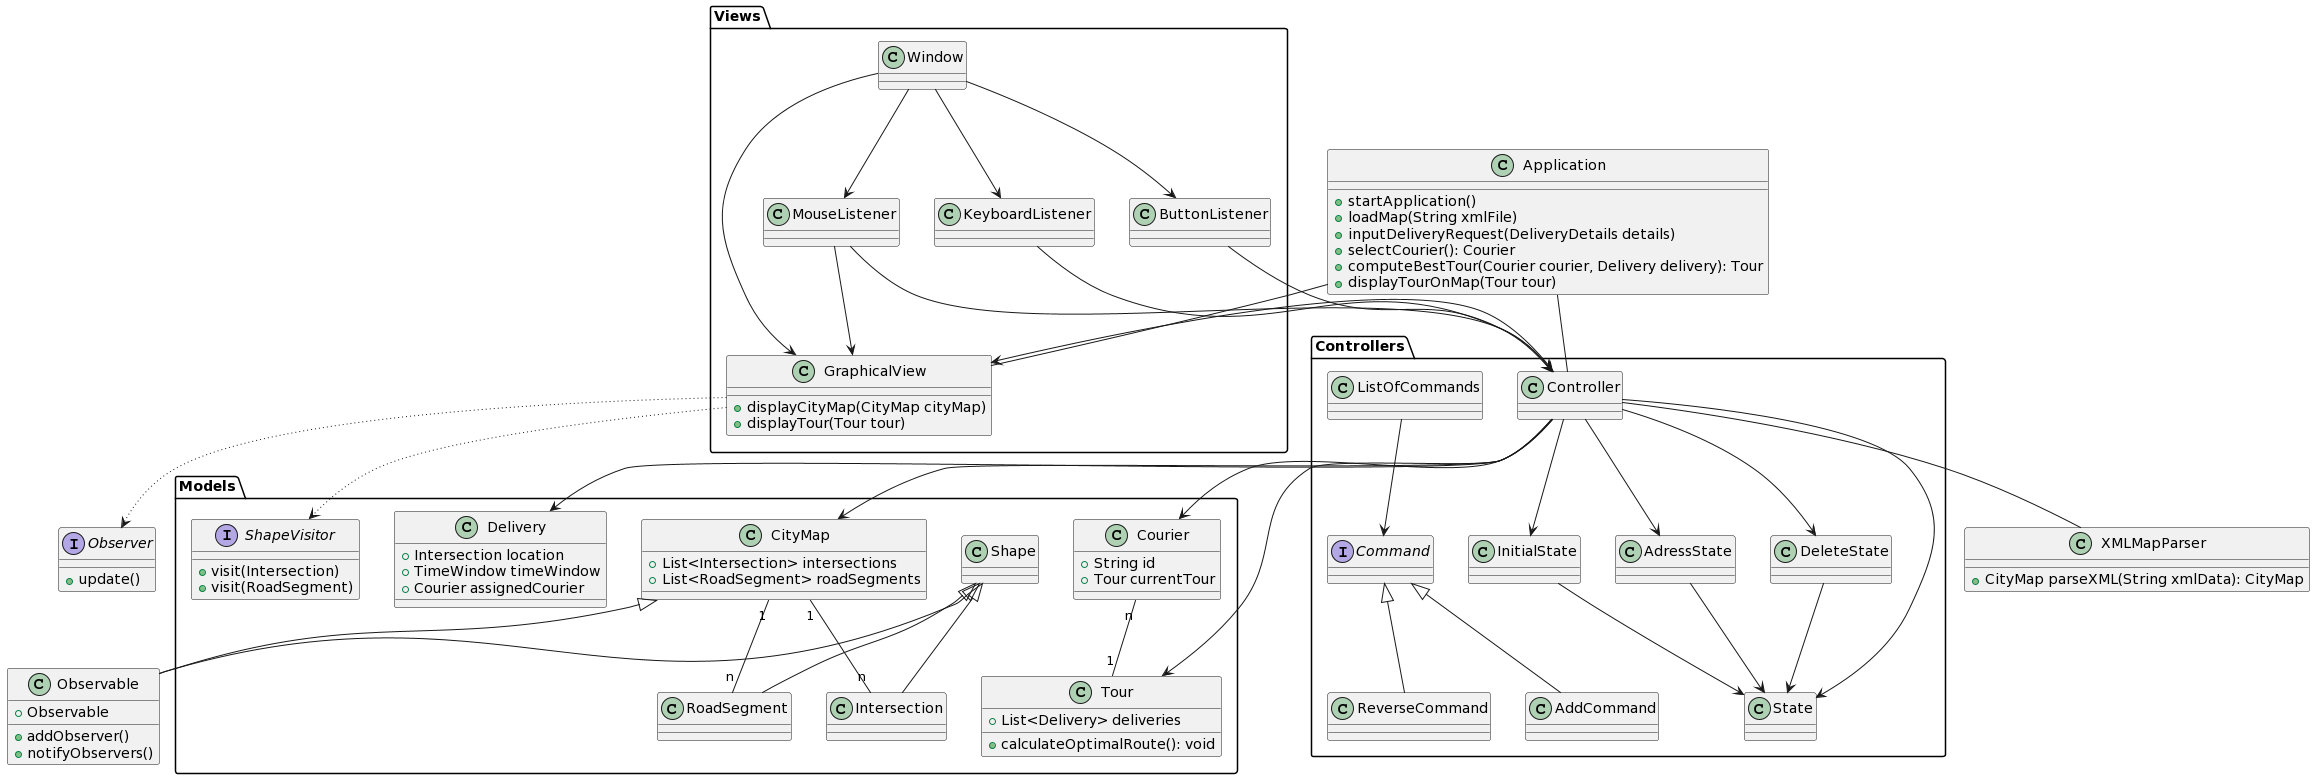
\includegraphics[width=\linewidth, height=\textheight, keepaspectratio]{architecture_diag.png}
\caption{Class and Package Diagram}
\end{figure}
\end{landscape}

\subsection{Sprint Planning}
For a sprint planning for a team of seven members over four sessions, focusing on the inception phase of your project, it's important to allocate tasks effectively to meet all deliverables. We had 4 Sessions with 4 hours per session. Here's a suggested sprint plan:

\subsubsection*{Session Breakdown and Task Allocation:}

\paragraph{Session 1:}
\begin{itemize}
    \item \textbf{All Members}: Setting up project environment for development and conception. - 2 hours per member
    \item \textbf{All Members}: Brainstorming session for identifying main use cases and initial architecture. - 1 hour per member
    \item \textbf{Tim}: Start working on the Glossary. - 1 hour
    \item \textbf{Marie \& Noham}: Use Case Diagram. - 1 hour
    \item \textbf{Mark \& Hugo}: Sequence and Class Diagram. - 1 hour
    \item \textbf{Evann}: Architecture conception - 1 hour
    \item \textbf{Zyad}: Sick
\end{itemize}

\paragraph{Session 2:}
\begin{itemize}
    \item \textbf{All members}: Daily discussion on where everybody is at. Synthesis of 1st session results. - 30 min
    \item \textbf{Evann \& Hugo}: Continuation of architecture conception. - 3h
    \item \textbf{Marie and Noham}: Structured description of selected use cases. - 1.5h
    \item \textbf{Noham}: Joined Mark to work on algorithms. - 1.5h
    \item \textbf{Tim \& Zyad}: Conception of UX/UI. - 3h
    \item \textbf{Marie}: Joined the front end team to design and program the UI. - 1.5h
    \item \textbf{Mark}: Research on algorithms and look at given code for TSP. - 3h
    \item \textbf{All Members}: Recapitulative Discussion. - 30 min
\end{itemize}

\paragraph{Session 3:}
\begin{itemize}
    \item \textbf{All members}: Daily discussion on where everybody is at. Synthesis of 1st session results. - 30 min
    \item \textbf{All members}: Revisited packages, validation and implementation of packages and classes. - 2h
    \item \textbf{Mark \& Hugo \& Noham \& Evann}: Continued work on algorithms. - 1.5h
    \item \textbf{Marie \& Tim}: Front End Development - Correction of bugs related to displaying and the UI. - 1.5h
    \item \textbf{Hugo \& Evann}: Debugging Git. - 1h
    \item \textbf{All Members}: Recapitulative Discussion. - 10 min
\end{itemize}

\paragraph{Session 4:}
\begin{itemize}
    \item \textbf{All members}: Daily discussion on where everybody is at. Synthesis of 1st session results. - 30 min
    \item \textbf{Noham \& Evann}: Debugging backend. - 1.5h
    \item \textbf{Hugo \& Zyad \& Tim}: Front End Debugging and background improvement. - 1.5h
    \item \textbf{All Members}: Class meeting. - 2.5h
    \item \textbf{Marie \& Mark}: Developing deliverables. - 1.5h
\end{itemize}

\paragraph{Outside Sessions work:}
\begin{itemize}
    \item \textbf{Tim}: Development of V1 XML parser. - 2h
    \item \textbf{Marie}: Development of map for UI. - 3h
    \item \textbf{All Members}: Backend development and Code Cleaning. - 5h per member
\end{itemize}

\section{Important for Next Iterations}

We chose to take some more advanced decisions when it comes to architecture and design patterns in the first iteration of our project in order to start developing clean code with the right structure when it comes to packages, patterns, and classes. The following part will discuss the decisions we took for this. When it comes to architecture, packages, patterns, and classes, you can have a look at them in our Package and Class diagram.

\subsection{Architecture Choice}

The application employs the Model-View-Controller (MVC) architecture, providing several advantages:

\begin{itemize}
    \item \textbf{Separation of Concerns}: MVC divides the application into three main components—Model, View, and Controller—facilitating ease of maintenance and code evolution.
    \item \textbf{Ease of Maintenance}: Developers can work on individual components without affecting others. For example, UI design changes do not impact business logic.
    \item \textbf{Parallel Development}: Teams can work simultaneously on different components, accelerating development.
    \item \textbf{Code Reusability}: Models can often be reused across different views, and views with different controllers.
    \item \textbf{Ease of Testing}: Clear separation simplifies unit testing and debugging. Components can be tested independently.
    \item \textbf{Data Presentation Flexibility}: The separation allows the same data to be presented in different ways, useful for applications requiring diverse UIs.
    \item \textbf{Adaptability and Scalability}: MVC provides flexibility to evolve and adapt the application to changing needs without a complete overhaul.
    \item \textbf{Complex Interaction Handling}: Efficient management of complex interactions between UI and business logic, crucial for modern web applications.
\end{itemize}

\subsection{Unit Testing with JUnit}

For unit testing, we will use JUnit, Mockito, and JFixture. Here is a simplified example of a unit test in Java using JFixture for test data generation and Mockito for mocking dependencies:

\subsubsection*{Example for the Classes:}
\begin{verbatim}
public class UserService {
    private UserRepository userRepository;

    public UserService(UserRepository userRepository) {
        this.userRepository = userRepository;
    }

    public User getUserById(String userId) {
        return userRepository.findById(userId);
    }
}

public interface UserRepository {
    User findById(String userId);
}

public class User {
    private String id;
    private String name;
    // Getters, setters, etc.
}
\end{verbatim}

\subsubsection*{Example of Unitary Tests:}
\begin{verbatim}
import static org.mockito.Mockito.*;
import static org.junit.Assert.*;
import org.junit.Before;
import org.junit.Test;
import com.flextrade.jfixture.JFixture;

public class UserServiceTest {

    private UserRepository userRepositoryMock;
    private UserService userService;
    private JFixture fixture;
    private String userId;
    private User expectedUser;

    @Before
    public void setUp() {
        // Création d'un mock pour UserRepository
        userRepositoryMock = mock(UserRepository.class);
        
        // Initialisation de UserService avec le mock
        userService = new UserService(userRepositoryMock);

        // Initialisation de JFixture pour la génération de données
        fixture = new JFixture();
        
        // Création d'un ID utilisateur et d'un objet User
        userId = fixture.create(String.class);
        expectedUser = fixture.create(User.class);
        
        // Configuration du comportement du mock
        when(userRepositoryMock.findById(userId)).thenReturn(expectedUser);
    }

    @Test
    public void getUserById_ShouldReturnUser() {
        // Action: Appel de la méthode à tester
        User result = userService.getUserById(userId);

        // Vérification: Le résultat doit correspondre à l'objet User attendu
        assertEquals(expectedUser, result);

        // Vérification que le mock a été appelé comme prévu
        verify(userRepositoryMock).findById(userId);
    }
}
\end{verbatim}

In this example, JFixture is used for automatic instance creation, and Mockito for mocking UserRepository and configuring its behavior. The test verifies that \texttt{userService.getUserById} returns the expected User object and that the mock repository is called correctly.


\section{Glossary}

\begin{enumerate}
    \item \textbf{\textit{Application}}: The software system designed for optimizing delivery tours in cities using bicycles.
    \item \textbf{\textit{City Map}}: A digital representation of a city's layout, including intersections and road segments, used for planning delivery tours.
    \item \textbf{\textit{Intersection}}: A point where two or more roads meet in the city map, characterized by its geographical coordinates: latitude and longitude.
    \item \textbf{\textit{Latitude}}: The geographic coordinate that specifies the north-south position of a point on the Earth's surface.
    \item \textbf{\textit{Longitude}}: The geographic coordinate that specifies the east-west position of a point on the Earth's surface.
    \item \textbf{\textit{Road Segment}}: A stretch of road connecting two intersections, with attributes like origin, destination, name, and length.
    \item \textbf{\textit{XML File}}: A file format used to describe the city map, including details of intersections, road segments, and the warehouse address.
    \item \textbf{\textit{Warehouse}}: The starting and ending point for courier tours, where deliveries are dispatched from.
    \item \textbf{\textit{Courier}}: An individual responsible for carrying out deliveries on a bicycle.
    \item \textbf{\textit{Delivery Request}}: An order for goods to be delivered to a specific location within a designated time-window.
    \item \textbf{\textit{Time-Window}}: A specified duration, here, one hour, within which a delivery must be made. Starts at fixed hours in the morning (8, 9, 10, or 11 a.m.).
    \item \textbf{\textit{Tour}}: A sequence of deliveries assigned to a courier, including start and end times, delivery locations, and time-windows.
    \item \textbf{\textit{Tour Optimization}}: The process of determining the most efficient route for a courier to complete all assigned deliveries within their time-windows.
    \item \textbf{\textit{Address}}: The specific location for a delivery, typically including details like street name, number, city, and sometimes latitude and longitude coordinates.
    \item \textbf{\textit{Travel Speed}}: The assumed constant speed of the couriers, used for calculating tour durations and feasibility.
    \item \textbf{\textit{Delivery Performance Time}}: The time taken to perform a delivery, assumed to be a constant (e.g., five minutes).
    \item \textbf{\textit{User}}: The person operating the application, responsible for loading maps, inputting delivery requests, and managing couriers.
    \item \textbf{\textit{Manager UberIF}}: The user that gets incoming delivery requests, calculates routes from the warehouse, and manages the couriers.
\end{enumerate}


\end{document}
